\section{Conception}

\subsection{Délimitation fonctionnelle}

La figure \ref{fig:delimitation_fonctionnelle} illustre la délimitation fonctionnelle du contrôleur I2C. La délimitation fonctionnelle est définie par les relations d'entrées-sorties du composant. Le contrôleur I2C est un composant autonome qui communique avec l'entité Système à uP et l'entité Esclave distant via ces relations.

\begin{figure}[H]
    \centering
    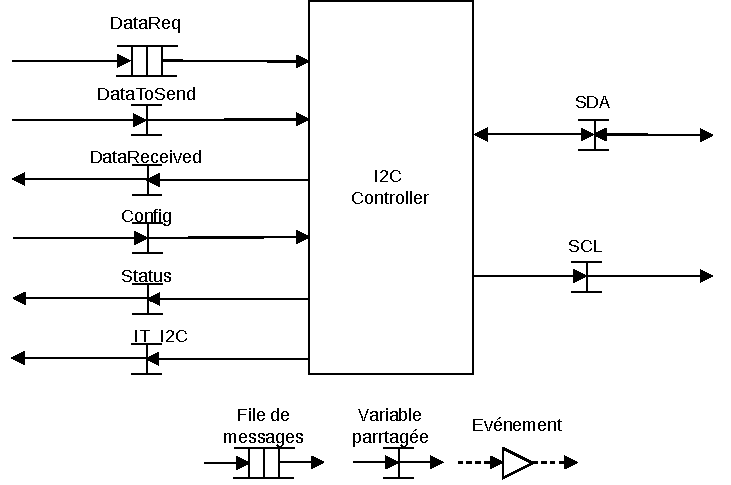
\includegraphics[width=0.95\linewidth]{Images/3_CONCEPTION/Délimitations entrées sorties.pdf}
    \caption{Délimitation fonctionnelle du contrôleur I2C}
    \label{fig:delimitation_fonctionnelle}
\end{figure}

\subsection{Introduction des interfaces}

Dans cette étape, on tient compte des signaux logiques qui sont échangés entre le contrôleur I2C et les entités Système à uP et Esclave distant. Ces signaux sont regroupés en interfaces. Une interface est un ensemble de signaux logiques qui sont échangés entre deux entités. Le contrôleur I2C possède deux interfaces : l'interface Système à uP et l'interface Esclave distant.

\begin{figure}[H]
    \centering
    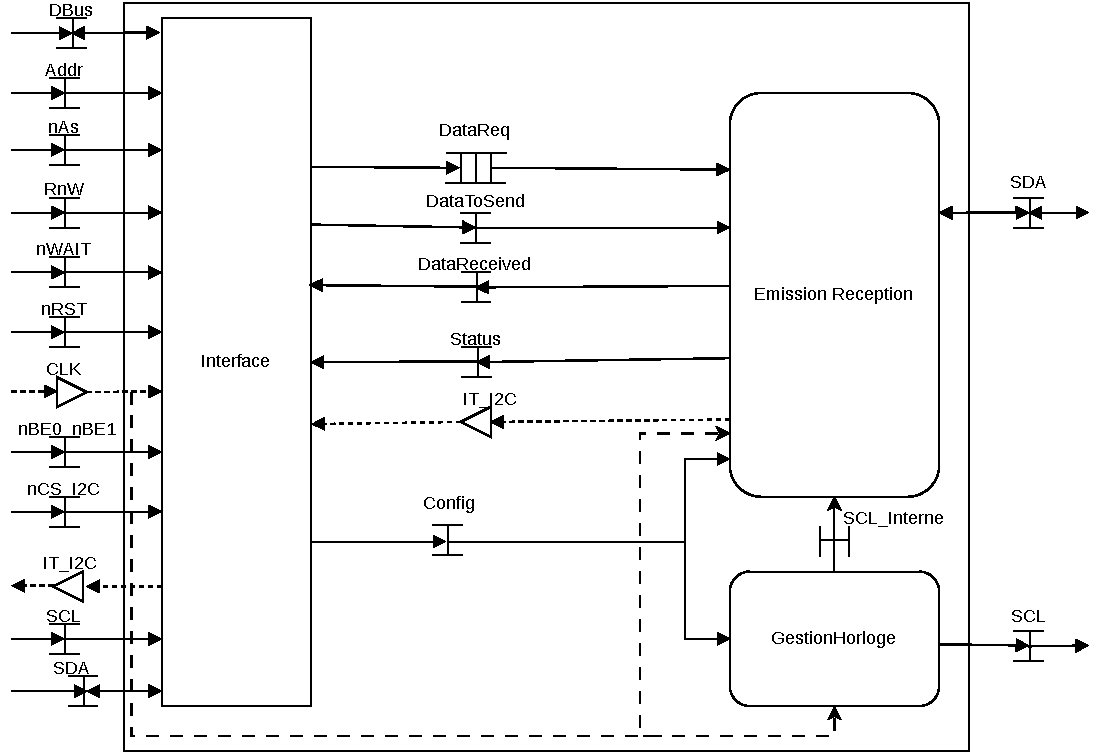
\includegraphics[width=0.95\linewidth]{Images/3_CONCEPTION/Solution fonctionnelle après intro des interfaces.pdf}
    \caption{Interfaces du contrôleur I2C}
    \label{fig:interfaces}
\end{figure}